\newcommand{\mgamcnlo}{MG5\_aMC@NLO\xspace}
\newcommand{\A}{A}

An important requirement for models of dark matter is their consistency with existing astrophysical observations, namely the observed dark matter relic density.
The relic density is driven by the annihilation cross-section of dark matter into SM particles.
For a given model of dark matter-SM interactions, the annihilation cross-section is fully defined and a calculation of the resulting relic density can be performed. 

\subsection{Technical setup}
The \maddm~\cite{Backovic:2013dpa,Backovic:2015cra} plugin for \mgamcnlo is used to calculate the present-day relic density for this model.
By modeling the thermal evolution of the cross-section during the expansion of the early universe, the time of freeze-out is determined.
All tree-level annihilation processes are taken into account, and the Yukawa couplings of all fermions are taken to be non-zero.
The Feynman diagrams of annihilation processes taken into account in this calculation are shown in Fig.~\ref{fig:feyn_annihilation}. Generally, the annihilation proceeds via single or double s-channel exchange of the pseudoscalars a and A, with subsequent decays. Since \maddm uses only tree-level diagrams, contributions from off-shell pseudoscalars can only be taken into account for the case of single s-channel mediation with direct decay of the pseudoscalar to SM fermions. If the pseudoscalar instead decays to other bosons or if the annihilation proceeds through double s-channel diagrams, the outgoing bosons are taken to be on-shell and their decays are not simulated. 

\subsection{Results}
The relic density is shown for a scan in the \ma-\mDM plane in Fig.~\ref{fig:relic_scan_mxd_ma}.
For small values of $\mDM$ below the mass of the top quark, DM is mostly overabundant. In this regime, annihilation to quarks is suppressed by the small Yukawa couplings of the light fermions. The observed relic density can only be achieved for $\mDM\approx\ma/2$, where annihilation is resonantly enhanced, or for $\mDM \approx (\ma+\mh)/2$, close to the threshold for the $\chi\chi\rightarrow h a$ process.
Above the top threshold, annihilation into fermions becomes very efficient and DM is underabundant. As \mDM increases further, annihilation via single s-channel diagrams is increasingly suppressed and the relic density rises again. The observed density is reproduced again for $\mDM\approx1 \mathrm{TeV}$ at low \ma.
For values of \ma beyond the LHC reach of a few TeV, the allowed parameter region at the top threshold $\mDM\approx m_{\mathrm{top}}$ stays independent of the value of \ma, indicating that a DM candidate that is mass degenerate with the top quark cannot be excluded by LHC searches alone.

The dependence of the relic density on the choice of \mDM is further explored by performing a one-dimensional scan, as shown in Fig.~\ref{fig:relic_scan_mxd}. The relic density shows clear structures corresponding to the previously discussed regions of resonant enhancement, as well as kinematic boundaries. Overall, the behavior is dominated by the low-\mDM suppression of the annihilation cross-section, the reosnant enhancement at $\mDM = \ma/2$ and the kinematic top thresholds. Other effects, such as resonant enhancement of $\chi\chi\rightarrow A$ annihilation are present, but only have small effects.

\begin{figure}[h]
\centering
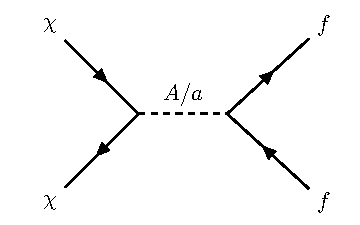
\includegraphics[width=0.35\textwidth]{texinputs/05_relic/figures/feynman/graph_2hdm_relic_s_fermions.pdf}
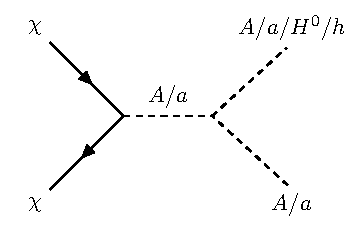
\includegraphics[width=0.35\textwidth]{texinputs/05_relic/figures/feynman/graph_2hdm_relic_s_bosons.pdf}
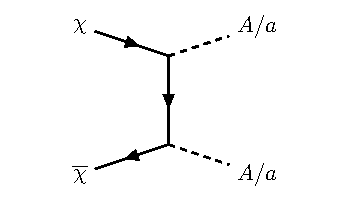
\includegraphics[width=0.35\textwidth]{texinputs/05_relic/figures/feynman/graph_2hdm_relic_ss_bosons.pdf}
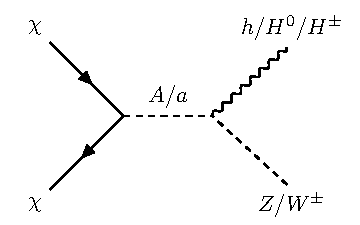
\includegraphics[width=0.35\textwidth]{texinputs/05_relic/figures/feynman/graph_2hdm_relic_s_vbosons.pdf}

\caption{Annihilation diagrams taken into account in the relic density calculation.}
\label{fig:feyn_annihilation}
\end{figure}

\begin{figure}[h]
\centering
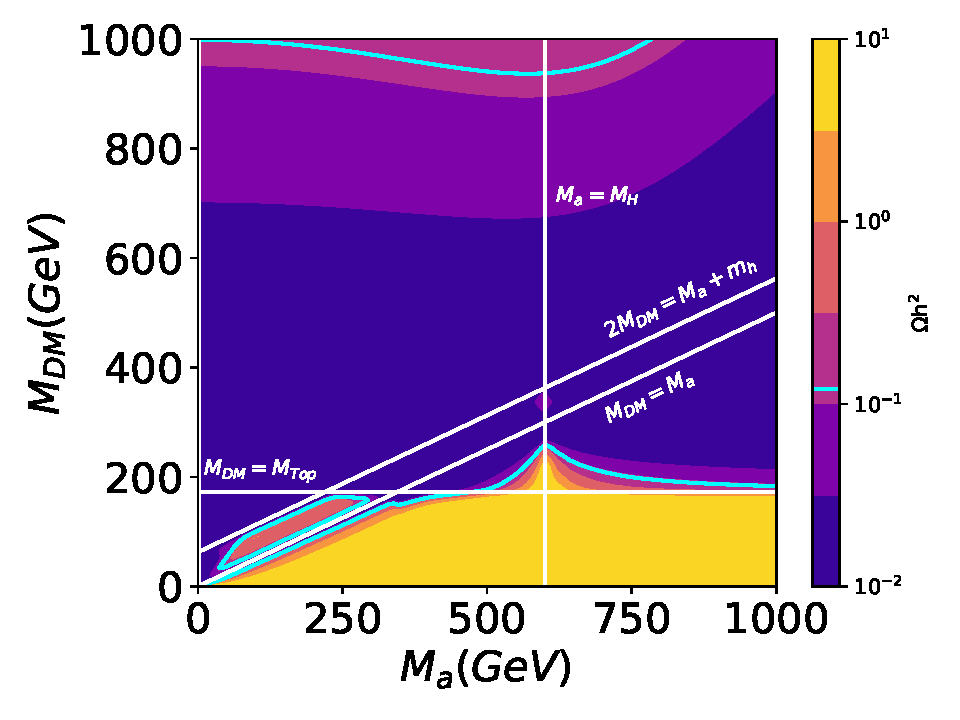
\includegraphics[width=0.49\textwidth]{{texinputs/05_relic/figures/relic/contour_scan_mxd_ma.pdf}}
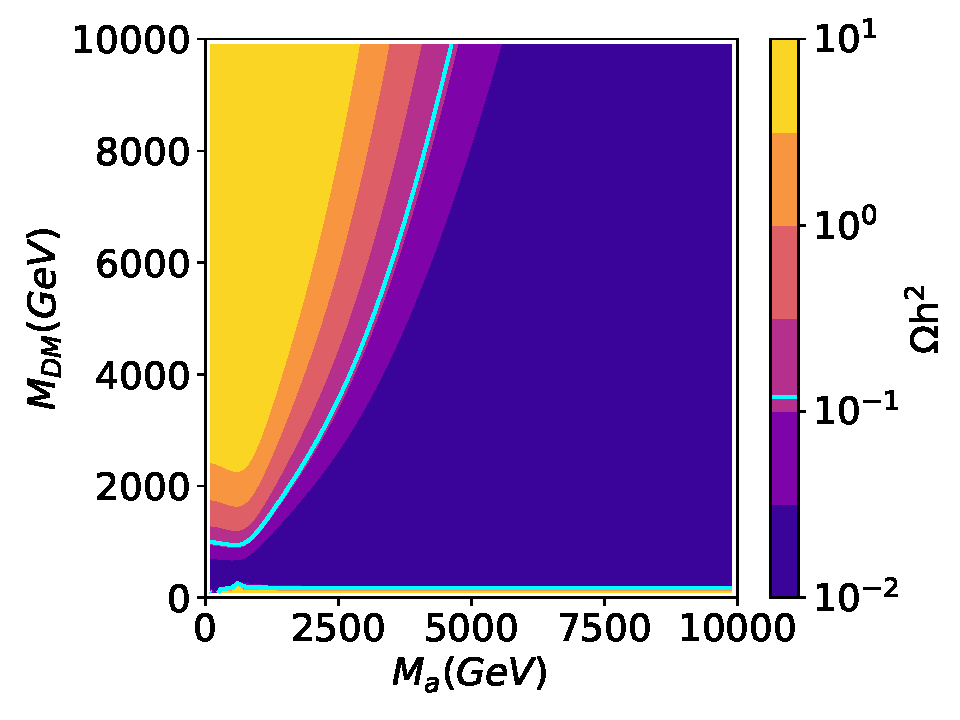
\includegraphics[width=0.49\textwidth]{{texinputs/05_relic/figures/relic/contour_scan_mxd_ma_large.pdf}}


\caption{Predicted relic density for a two-dimensional scan of \mDM and \ma. The color scale indicates the relic density, the cyan solid line shows the observed value of $\Omega h^{2} = 0.12$. The color scale is truncated at its ends, i.e. values larger than the maximum or smaller than the minimum are shown in the same color as the maximum/minimum. While the left focuses on the mass region relevant to collider searches, the right panel shows the development of the relic density for a larger mass region.}
\label{fig:relic_scan_mxd_ma}
\end{figure}

\begin{figure}[h]
\centering
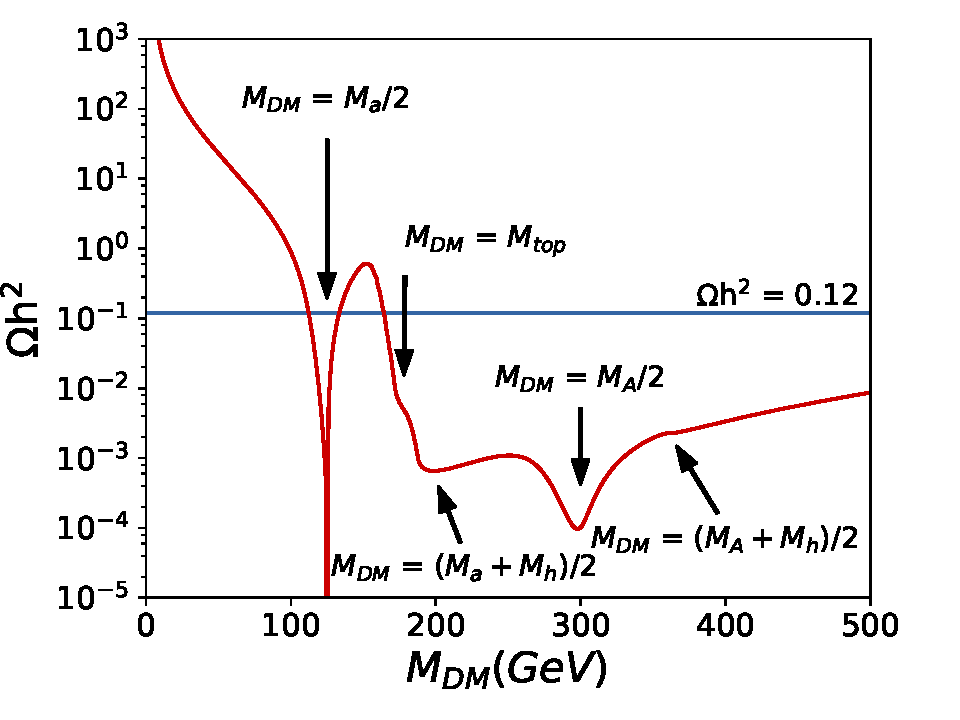
\includegraphics[width=0.8\textwidth]{texinputs/05_relic/figures/relic/line_scan_mdm.pdf}
\caption{Relic density for a one-dimensional scan of \mDM. Various kinematic thresholds and regions of resonant enhancement are visible. Consistency with the observed value of $\Omega h^{2} = 0.12$ is mainly controlled by the resonant enhancement of $\chi\chi\rightarrow a$, as well as the onset of $\chi\chi\rightarrow t\overline{t}$.}
\label{fig:relic_scan_mxd}
\end{figure}
